\chapter{Aplikacja sterująca}
\label{cha:aplikacja_sterujaca}
W niniejszym rozdziale przedstawiono informacje na temat aplikacji sterującej. Zagadnienia teoretyczne konieczne do zrozumienia problemu, poszczególne etapy przygotowania platformy sprzętowej, oraz proces tworzenia systemu czasu rzeczywistego.




\section{System czasu rzeczywistego}
System czasu rzeczywistego (ang. real-time system) to system, który przetwarza każdy rodzaj informacji i który musi reagować na sygnały wejściowe - bodźce generowane z zewnątrz w skończonym i określonym czasie. Jego poprawne działanie zależy zarówno od prawidłowych rezultatów logicznych, jak również od czasu reakcji.
Na podstawie tych kryteriów są one dzielone na:
\begin{itemize}
	\item Systemy o ostrych wymaganiach czasowych (ang. hard real-time) - wymagania czasowe muszą być skrupulatnie przestrzegane, naruszenie ram czasowych może wpłynąć na życie ludzkie, środowisko czy też sam system,
 
	\item Systemy o słabych wymaganiach czasowych (ang. soft real-time) – głównym kryterium oceny tych jest średni czas odpowiedzi. Sporadyczne opóźnienie nie powoduje zagrożenia lecz jedynie wpływa negatywnie na ocenę całego systemu,

	\item Systemy o solidnych wymaganiach czasowych (ang. firm real-time) - są one kombinacją systemów o wymaganiach ostrych oraz słabych. Naruszenie kryterium czasowych może pojawiać się okazjonalnie. Często dla lepszej oceny systemu stosuje się ograniczenia czasowe o charakterze "słabym" - krótsze, których przekroczenie nie powoduje katastrofy oraz "ostrym" - dłuższe, których naruszenie oznacza nieprawidłowe działanie systemu. 

\end{itemize}

Bez względu na to do której grupy systemów zalicza się aplikację musi ona charakteryzować się następującymi cechami:

\begin{itemize}
	\item Ciągłość działania - powinny działać nieprzerwanie w okresie od uruchomienia systemu do jego wycofania,
	
	\item Zależność od otoczenia - zachowanie opiera rozpatruje się w kontekście otoczenia. Prowadzone obliczenia zależą od zdarzeń oraz danych pochodzących z zewnątrz układu,
	
	\item Współbieżność - struktura systemu narzuca, aby jednoczesne zdarzenia były obsługiwane równocześnie przez szereg procesów,
	
	\item Przewidywalność - zdarzenia i dane generowane przez otoczenie pojawiają się przypadkowo co nie narusza deterministycznego zachowania systemu,
	
	\item Punktualność - odpowiedź systemu na bodźce zewnętrzne powinna być dostarczona w odpowiednich momentach - wymaganych ramach czasowych.
\end{itemize}

Z pewnością aplikacja sterująca obiektami latającymi powinna spełniać wszystkie powyższe założenia. Gdyby któreś z nich nie zostało spełnione jakiekolwiek próby sterowania zakończyły by się porażką.

Dynamika wielokomórkowców wymaga od aplikacji bardzo szybkiego czasu reakcji na zewnętrzne impulsy. Opóźnienie sterowania w takim przypadku powoduje bardzo negatywne skutki do których zaliczamy: brak kontroli nad obiektem, utrata stabilności w powietrzu oraz niekontrolowane zetknięciu się z przeszkodą. Wszystkie wymienione zachowania mogą powodować bardzo duże zniszczenia dla modelu, jego otoczenia oraz zagrażać zdrowiu operatora oraz innych osób znajdujących się w zasięgu działania modelu.

Na podstawie definicji oraz powyższej analizy skutków określono, iż aplikacja sterującą zalicza się do systemu hard-real time. 




\section{Konfiguracja beaglebone black}
Ze względu na kontynuację prac nad modelem bazowa konfiguracja beaglebone black wraz z dodatkowymi czujnikami oraz urządzeniami peryferyjnymi opisano w pracy
%TODO: inz Rwlodarz JZrebiec.

W trakcje powstawania niniejszej pracy na rynku dostępne są nowsze czujniki, które mogłyby podnieść jakość oraz częstość pomiarów, jednak ingerencja w konfigurację uniemożliwiła by porównanie algorytmów tradycyjnych z sieciami neuronowym stąd wszystkie testy zostały przeprowadzone na tej samej konfiguracji.




\section{Przygotowanie systemu operacyjnego}
Ze względu na wcześniej wspominaną specyfikę systemu sterującego oraz zastosowanie platformy sprzętowej typu mini PC wraz z systemem operacyjnym typu UNIX, ważne jest, aby wyeliminować wszelkie możliwe przerwania procesora oraz inne aspekty, które wpływają na płynność oraz czas wykonywania się aplikacji sterującej.

Wprowadzono usprawnienie w postaci instalacji systemu operacyjnego wyposażonego w jądro czasu rzeczywistego (ang. real-time kernel). Jądro to określane jest również jako w pełni wywłaszczalne. Oznacza to, iż dopuszczane jest wywłaszczenie procesu działającego w trybie jądra. Cecha ta wraz z wcześniej narzuconymi priorytetami dla poszczególnych procesów gwarantuje, iż aplikacja sterująca, uruchomiona z wysokim priorytetem nie zostanie wywłaszczona na zbyt długi czas przez inne procesy systemowe.


Zabieg ten pozwala nam spełnić podstawową cechę systemów czasu rzeczywistego, którą jest punktualność.



\section{Architektura systemu sterującego}

Aplikacja sterująca ze względu na zastosowanie algorytmu opartego na sieciach neuronowych nie posiada dedykowanych rozwiązań pod konkretne zagadnienie. Jej budowa opiera się na tworzeniu sztucznej sieci neuronowej oraz dostarczeniu niezbędnych do jej działania funkcji - wczytywania wag dla poszczególnych połączeń oraz algorytmu uczącego. Dodatkowo została ona rozbudowana o system logowania danych, który okazał się bardzo pomocny w wykrywaniu nieprawidłowości w działaniu aplikacji oraz dostarcza dane niezbędne do dogłębnej analizy zagadnienia.

W celu dokładnego zrozumienia architektury oraz szczegółów związanych z implementacją poniżej przedstawiono szczegółowy opis poszczególnych elementów aplikacji:
\begin{itemize}
	\item klasa Neuron - jest to najważniejszy element w aplikacji. Jest on odpowiedzialny za przekazywanie odpowiednio przetworzonego sygnału z jego wejść na wyjście. Dodatkowo znajdują się w nim konieczne do realizacji algorytmu propagacji wstecznej informacje oraz funkcje. Posiada dostęp do wartości współczynników $\eta$ oraz $\alpha$, które są niezbędne do parametryzowania 
	
	
	Został on również wyposażony w indeks, który odpowiada jego miejscu w warstwie. Nie jest to informacje konieczna do poprawnego działania sieci jednak zdecydowanie ułatwia podgląd przepływu informacji przez sieć neuronową.  
	\item klasa Net - odpowiada za pełną reprezentację sieci. Przechowuje w wektorze wszystkie utworzone neurony w uszeregowanych warstwach. W swoim konstruktorze przyjmuje wektor liczb, które odpowiadają za liczbę tworzonych warstw oraz ilości neuronów w każdej z nich. W zależności od konfiguracji inicjowane są wagi wszystkich połączeń. Są one dobierane losowo lub za pomocą wcześniej zdefiniowanych wartości. Wywołanie funkcji feedForward z argumentem w postaci wektora danych wejściowych powoduje przepływ i przetworzenie informacji przez sieć. Wektor wartości wyjściową odczytujemy za pomocą funkcji getResults. Dodatkowo klasa ta została wyposażona w funkcje backProp, która odpowiada za uczenie sieci metodą propagacji wstecznej. 
	\item kontener Layer - dla lepszego zobrazowania struktury aplikacji neurony reprezentujące poszczególną warstwę są przechowywane w wektorze. 
	\item struktura Connection - odpowiada za przejrzystą reprezentację synaps w układzie biologicznym. Przetrzymuje ona informacje na temat wagi połączenia, które reprezentuje oraz wartość modyfikacji z procesu uczenia.
	\item klasa Logger - ze względu na ostre wymagania czasowe utworzono asynchroniczny logger z konfigurowalnymi poziomami logowania. Jego użycie wymaga wywołania funkcji addMsg do której podajemy argument świadczący o priorytecie informacji ERROR, WARNING, INFORMATION, DEBUG oraz jej treści jako następny argument. Wiadomość ta jest dodawana do kolejki, która jest cyklicznie wypisywana do pliku w niezależnym wątku. Zabieg ten pozwala na zabezpieczenie przed ewentualnym przyblokowaniem głównego wątku sterującego w przypadku problemów z dostępem do pliku lub innych nieprawidłowości. Istnieje również możliwość konfiguracji poziomu logowania, jest znacząca cecha w przypadku systemów czasu rzeczywistego. Podczas testów warto posiadać wszystkie informacje na temat działania systemu jednak po ich ukończeniu są one zbędne w przypadku normalnego użytkowania, kiedy istotne są jedynie te informacje które świadczą o błędach w systemie. Nadmiar logowanych danych wpływa negatywnie na czas wykonywania się pętli sterowania oraz przechowywane dane zajmują sporo pamięci w przypadku systemów wbudowanych.
	Całość została obudowana w wzorzec projektowy Singleton, aby ułatwić dostęp do klasy oraz zabezpieczyć kod przed utworzeniem wielu instancji tego obiektu.
\end{itemize}


\begin{sidewaysfigure}[ht]
\centering
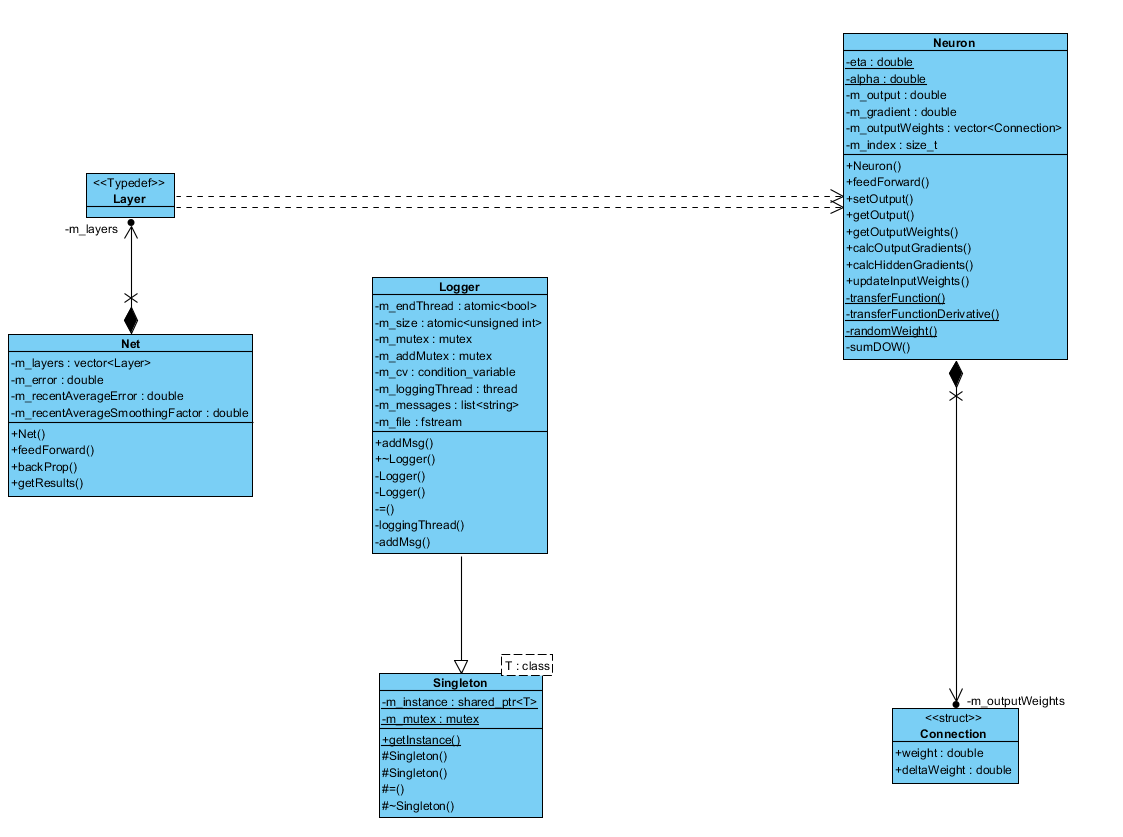
\includegraphics[width=0.7\linewidth]{./include/diagram}
\caption{Diagram klass aplikacji sterującej.}
\label{fig:diagram}
\end{sidewaysfigure}

\section{Niezależność aplikacji od platformy sprzętowej}
Dobrze zaprojektowana aplikacja sterująca obiektami latającymi powinna mieć możliwość uruchomienia na różnorodnych platformach sprzętowych, bez względu na architekturę wykorzystanych procesorów. Ponieważ, zagadnienie to jest obszerne autor zdecydował się wyszczególnić jedynie najważniejsze aspekty związane z przenoszeniem kodu napisanego w języku C++ pomiędzy platformami. 

Na podstawie analizy dokonanej przez autora w wybrano najważniejsze zagadnienia, które powodują różne działania aplikacji w zależności od systemu:
\begin{itemize}
	\item przechowywanie wartości typu integer pod typem double - w systemach 32 bitowych nie występował problem reprezentacji liczb całkowitych przez typ double. Standard języka C++ definiuje, iż zmienna ta posiada do 52 bitów zarezerwowanych na reprezentację takiej liczby. Warto jednak mieć na uwadze, iż w przypadku systemów 64 bitowych liczby całkowite przetrzymywane w typie size\_t posiadają, aż 64 bity przeznaczone do reprezentacji jej zawartości natomiast liczba bitów w przypadku typu double się nie zmienia. Problem ten prowadzi do niepoprawnej reprezentacji wartości całkowitych zajmujących ponad 52 bity przypisywanych do typu double. Wartość ta zostanie obcięta o początkowe 12 bitów. Zaleca się unikanie takich przypisań.
	
	\item operacje przesunięć bitowych - aplikacje dedykowane na systemy wbudowane często wykorzystują niskopoziomowe operacje takie jak przesunięcia bitowe. Przesunięcie bitowe liczby 0x00000001 o 32 miejsca w lewą stronę powoduje różne wyniki z zależności od architektury procesora. W przypadku systemu x86 otrzymamy wartość 0x00000000, a system x64 zwróci 0x00000000100000000. W przypadku odczytu takich wartości może to zdecydowanie wpłynąć na działanie aplikacji. Problem ten często rozwiązywany jest za pomocą definiowanie maksymalnego przesunięcia w pliku nagłówkowym - o 32 lub 64 bity w zależności od systemu.
	
	\item operacje mnożenia liczb zmiennoprzecinkowych -  operacja ta jest bardzo znanym zagadnieniem dającą odmienne wyniki z zależności od ilości bitów przewidzianych na poszczególną z liczb oraz wynik do którego przypisywany jest iloczyn. Ma to związek z uzyskaniem błędu odcięcia w przypadku nie wystarczającej liczbie bitów potrzebnych do reprezentacji części ułamkowej.
\end{itemize}

Na podstawie powyższych przykładów można zauważyć, iż możliwe jest stworzenie aplikacji której kod można przenosić pomiędzy różnymi architekturami. Nie mniej jednak warto zauważyć, że wymaga to sporo wiedzy na temat wykorzystywanych narzędzi oraz umiejętnego wykonywania wszelakich operacji na liczbach. Podejście to pozwala z wyeliminować błędy związane z dwoma pierwszym zagadnieniami. Trzeci problem wymaga jednak sprzętowego lub programowego zabezpieczenia przed tego typu zagrożeniami. Ze względu na ostatnie zagadnienie do implementacji sieci neuronowej wybrano język C++. Posiada on zdefiniowany standard, który gwarantuje, iż bez względu na system operacje zmiennoprzecinkowe na typach double gwarantują uzyskanie tego samego wyniku. Jest to bardzo ważne cecha, która zaważyła na tym, iż omawiana aplikacja została stworzona właśnie w tym języku. Warto mieć jednak na uwadze, iż operacje pomiędzy różnymi typami np. iloczyn float oraz double może powodować już komplikacje stąd należy ich unikać.

Podstawowa wersja aplikacji została poddana testom, które przez porównanie wyników działania sieci neuronowej na 2 całkowicie odmiennych platformach stanowią informację o możliwości stosowania implementacji na różnych systemach.
 
\subsection{Testy}
Do testów wykorzystano komputer stacjonarny z 64 bitowym procesorem Intel i5-4670 3.40 Ghz oraz układ beaglebone black, który został wyposażony w procesor 32 bitowy ARM Cortex-A8 o częstotliwości taktowania 1GHz.

W celu uwydatnienia problemu stworzono sieć neuronową posiadającą jedną  warstwę wejściową, ukrytą, wyjściową. Wagi poszczególnych neuronów zostały dobrane w sposób losowy. Konieczne jednak był dobór liczb, które maksymalnie wykorzystują precyzje liczby zmiennoprzecinkowej typu double. Następnie na wejście sieci podawana jest stała wartość oraz odczytywane jest wyjście sieci. Kroki te powtarzane są na  dostępnych platformach sprzętowych. Wyniki poszczególnych operacji są logowane, a następnie porównywane z ich odpowiednikami na innej platformie sprzętowej w celu zbadania rozbieżności.

Poniżej przedstawiono ogólny szkic testowanej topologi sieci z uwzględnieniem wag połączeń.

\section{Aplikacja sterująca}

Ze względu na powyżej omówione aspekty, do tworzenia aplikacji sterującej wykorzystano język C++. 

\begin{itemize}
	\item 1
	\item 2
	\item 3
	\item 4
	\item 5
	\item 6
\end{itemize}




